\documentclass{standalone}
\usepackage{tikz}
\usetikzlibrary{patterns, positioning}


\begin{document}
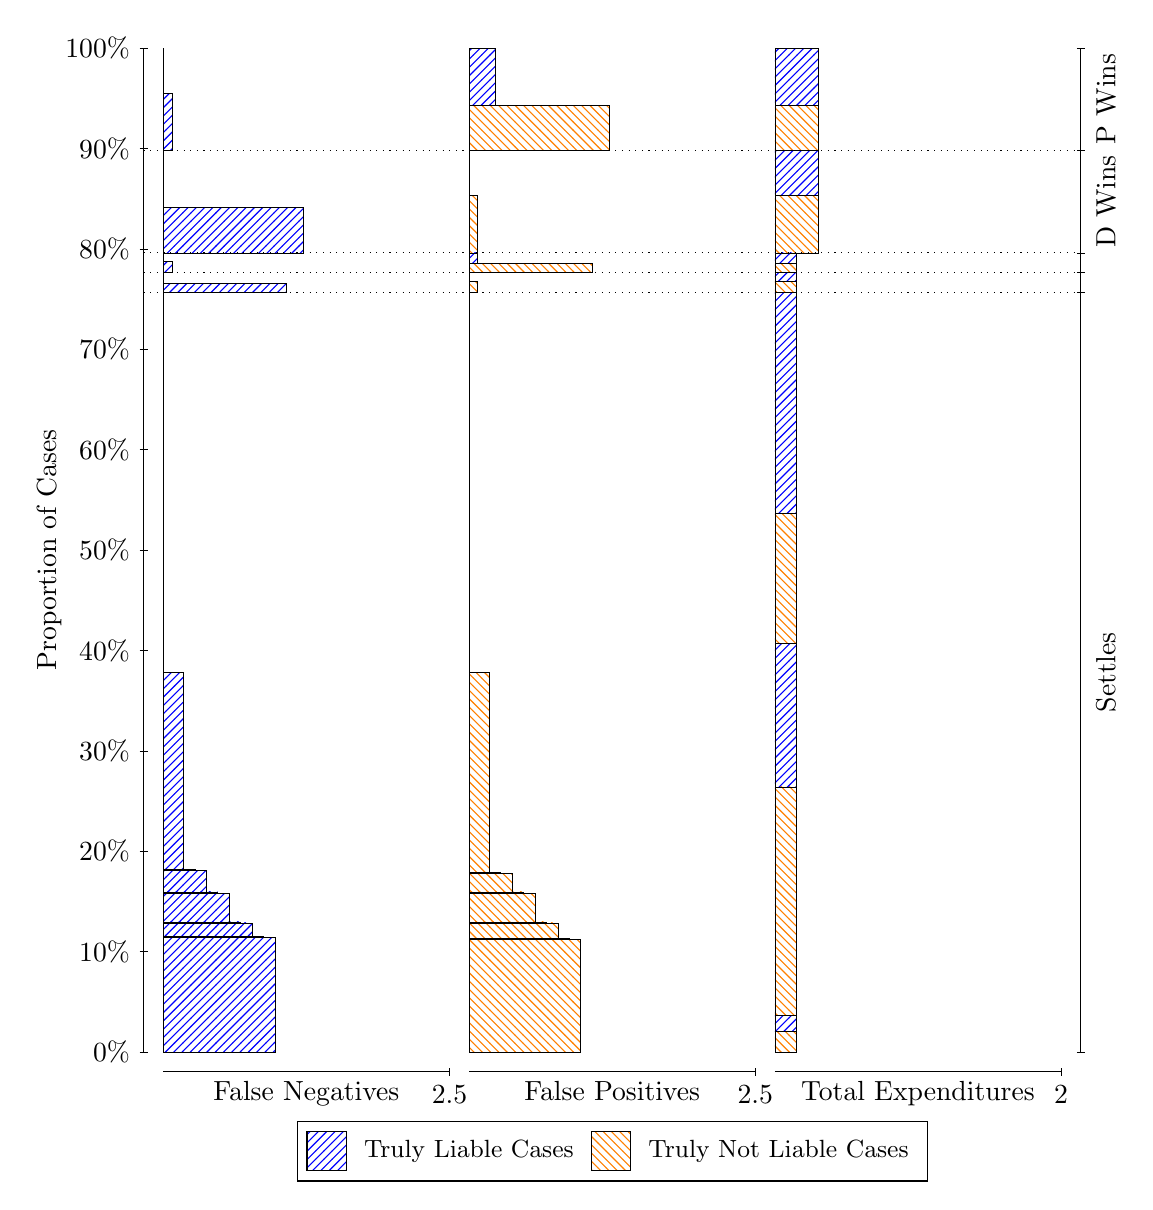
\begin{tikzpicture}
\draw[black, very thin] (1.5,1.75) -- (1.5,14.5);
\node[rotate=90, text=black, anchor=center] at (0.3, 8.125) {Proportion of Cases};
\draw[black, very thin] (1.45,1.75) -- (1.55,1.75);
\node[text=black, anchor=east] at (1.45, 1.75) {0\%};
\draw[black, very thin] (1.45,3.025) -- (1.55,3.025);
\node[text=black, anchor=east] at (1.45, 3.025) {10\%};
\draw[black, very thin] (1.45,4.3) -- (1.55,4.3);
\node[text=black, anchor=east] at (1.45, 4.3) {20\%};
\draw[black, very thin] (1.45,5.575) -- (1.55,5.575);
\node[text=black, anchor=east] at (1.45, 5.575) {30\%};
\draw[black, very thin] (1.45,6.85) -- (1.55,6.85);
\node[text=black, anchor=east] at (1.45, 6.85) {40\%};
\draw[black, very thin] (1.45,8.125) -- (1.55,8.125);
\node[text=black, anchor=east] at (1.45, 8.125) {50\%};
\draw[black, very thin] (1.45,9.4) -- (1.55,9.4);
\node[text=black, anchor=east] at (1.45, 9.4) {60\%};
\draw[black, very thin] (1.45,10.675) -- (1.55,10.675);
\node[text=black, anchor=east] at (1.45, 10.675) {70\%};
\draw[black, very thin] (1.45,11.95) -- (1.55,11.95);
\node[text=black, anchor=east] at (1.45, 11.95) {80\%};
\draw[black, very thin] (1.45,13.225) -- (1.55,13.225);
\node[text=black, anchor=east] at (1.45, 13.225) {90\%};
\draw[black, very thin] (1.45,14.5) -- (1.55,14.5);
\node[text=black, anchor=east] at (1.45, 14.5) {100\%};

\draw[black, very thin] (13.4,1.75) -- (13.4,14.5);
\draw[black, very thin] (13.35,1.75) -- (13.45,1.75);
\node[anchor=west] at (13.35, 1.75) {};
\draw[black, very thin] (13.35,11.394) -- (13.45,11.394);
\node[anchor=west] at (13.35, 11.394) {};
\draw[black, very thin] (13.35,11.65) -- (13.45,11.65);
\node[anchor=west] at (13.35, 11.65) {};
\draw[black, very thin] (13.35,11.899) -- (13.45,11.899);
\node[anchor=west] at (13.35, 11.899) {};
\draw[black, very thin] (13.35,13.2) -- (13.45,13.2);
\node[anchor=west] at (13.35, 13.2) {};
\draw[black, very thin] (13.35,14.5) -- (13.45,14.5);
\node[anchor=west] at (13.35, 14.5) {};

\draw[black, very thin, pattern color=blue, pattern=north east lines] (1.75,1.75) rectangle (3.167,3.205);
\draw[black, very thin, pattern color=blue, pattern=north east lines] (1.75,3.205) rectangle (3.0217,3.2142);
\draw[black, very thin, pattern color=blue, pattern=north east lines] (1.75,3.2142) rectangle (2.8763,3.3903);
\draw[black, very thin, pattern color=blue, pattern=north east lines] (1.75,3.3903) rectangle (2.731,3.4027);
\draw[black, very thin, pattern color=blue, pattern=north east lines] (1.75,3.4027) rectangle (2.5857,3.7663);
\draw[black, very thin, pattern color=blue, pattern=north east lines] (1.75,3.7663) rectangle (2.4403,3.7824);
\draw[black, very thin, pattern color=blue, pattern=north east lines] (1.75,3.7824) rectangle (2.295,4.0563);
\draw[black, very thin, pattern color=blue, pattern=north east lines] (1.75,4.0563) rectangle (2.1497,4.0687);
\draw[black, very thin, pattern color=blue, pattern=north east lines] (1.75,4.0687) rectangle (2.0043,6.5718);
\draw[black, very thin, pattern color=orange, pattern=north west lines] (1.75,6.5718) rectangle (1.75,11.394);
\draw[black, very thin, pattern color=blue, pattern=north east lines] (1.75,11.394) rectangle (3.3123,11.508);
\draw[black, very thin, pattern color=orange, pattern=north west lines] (1.75,11.508) rectangle (1.75,11.65);
\draw[black, very thin, pattern color=blue, pattern=north east lines] (1.75,11.65) rectangle (1.859,11.788);
\draw[black, very thin, pattern color=orange, pattern=north west lines] (1.75,11.788) rectangle (1.75,11.899);
\draw[black, very thin, pattern color=blue, pattern=north east lines] (1.75,11.899) rectangle (3.5303,12.475);
\draw[black, very thin, pattern color=orange, pattern=north west lines] (1.75,12.475) rectangle (1.75,13.2);
\draw[black, very thin, pattern color=blue, pattern=north east lines] (1.75,13.2) rectangle (1.859,13.925);
\draw[black, very thin, pattern color=orange, pattern=north west lines] (1.75,13.925) rectangle (1.75,14.5);
\draw[black, very thin, pattern color=orange, pattern=north west lines] (5.6333,1.75) rectangle (7.0503,3.1788);
\draw[black, very thin, pattern color=orange, pattern=north west lines] (5.6333,3.1788) rectangle (6.905,3.1879);
\draw[black, very thin, pattern color=orange, pattern=north west lines] (5.6333,3.1879) rectangle (6.7597,3.3902);
\draw[black, very thin, pattern color=orange, pattern=north west lines] (5.6333,3.3902) rectangle (6.6143,3.4032);
\draw[black, very thin, pattern color=orange, pattern=north west lines] (5.6333,3.4032) rectangle (6.469,3.7667);
\draw[black, very thin, pattern color=orange, pattern=north west lines] (5.6333,3.7667) rectangle (6.3237,3.77);
\draw[black, very thin, pattern color=orange, pattern=north west lines] (5.6333,3.77) rectangle (6.3237,3.7824);
\draw[black, very thin, pattern color=orange, pattern=north west lines] (5.6333,3.7824) rectangle (6.1783,4.0208);
\draw[black, very thin, pattern color=orange, pattern=north west lines] (5.6333,4.0208) rectangle (6.033,4.0331);
\draw[black, very thin, pattern color=orange, pattern=north west lines] (5.6333,4.0331) rectangle (5.8877,6.5718);
\draw[black, very thin, pattern color=blue, pattern=north east lines] (5.6333,6.5718) rectangle (5.6333,11.394);
\draw[black, very thin, pattern color=orange, pattern=north west lines] (5.6333,11.394) rectangle (5.7423,11.535);
\draw[black, very thin, pattern color=blue, pattern=north east lines] (5.6333,11.535) rectangle (5.6333,11.65);
\draw[black, very thin, pattern color=orange, pattern=north west lines] (5.6333,11.65) rectangle (7.1957,11.761);
\draw[black, very thin, pattern color=blue, pattern=north east lines] (5.6333,11.761) rectangle (5.7423,11.899);
\draw[black, very thin, pattern color=orange, pattern=north west lines] (5.6333,11.899) rectangle (5.7423,12.625);
\draw[black, very thin, pattern color=blue, pattern=north east lines] (5.6333,12.625) rectangle (5.6333,13.2);
\draw[black, very thin, pattern color=orange, pattern=north west lines] (5.6333,13.2) rectangle (7.4137,13.775);
\draw[black, very thin, pattern color=blue, pattern=north east lines] (5.6333,13.775) rectangle (5.9603,14.5);
\draw[black, very thin, pattern color=orange, pattern=north west lines] (9.5167,1.75) rectangle (9.7892,2.0164);
\draw[black, very thin, pattern color=blue, pattern=north east lines] (9.5167,2.0164) rectangle (9.7892,2.2141);
\draw[black, very thin, pattern color=orange, pattern=north west lines] (9.5167,2.2141) rectangle (9.7892,5.1164);
\draw[black, very thin, pattern color=blue, pattern=north east lines] (9.5167,5.1164) rectangle (9.7892,6.9349);
\draw[black, very thin, pattern color=orange, pattern=north west lines] (9.5167,6.9349) rectangle (9.7892,8.5881);
\draw[black, very thin, pattern color=blue, pattern=north east lines] (9.5167,8.5881) rectangle (9.7892,11.394);
\draw[black, very thin, pattern color=orange, pattern=north west lines] (9.5167,11.394) rectangle (9.7892,11.535);
\draw[black, very thin, pattern color=blue, pattern=north east lines] (9.5167,11.535) rectangle (9.7892,11.65);
\draw[black, very thin, pattern color=orange, pattern=north west lines] (9.5167,11.65) rectangle (9.7892,11.761);
\draw[black, very thin, pattern color=blue, pattern=north east lines] (9.5167,11.761) rectangle (9.7892,11.899);
\draw[black, very thin, pattern color=orange, pattern=north west lines] (9.5167,11.899) rectangle (10.062,12.625);
\draw[black, very thin, pattern color=blue, pattern=north east lines] (9.5167,12.625) rectangle (10.062,13.2);
\draw[black, very thin, pattern color=orange, pattern=north west lines] (9.5167,13.2) rectangle (10.062,13.775);
\draw[black, very thin, pattern color=blue, pattern=north east lines] (9.5167,13.775) rectangle (10.062,14.5);
\draw[black, dotted] (1.5,11.394) -- (13.4,11.394);
\draw[black, dotted] (1.5,11.65) -- (13.4,11.65);
\draw[black, dotted] (1.5,11.899) -- (13.4,11.899);
\draw[black, dotted] (1.5,13.2) -- (13.4,13.2);
\draw[black, very thin] (1.75,1.5) -- (5.3833,1.5);
\node[text=black, anchor=north] at (3.5667, 1.5) {False Negatives};
\draw[black, very thin] (5.3833,1.45) -- (5.3833,1.55);
\node[text=black, anchor=north] at (5.3833, 1.45) {2.5};

\draw[black, very thin] (5.6333,1.5) -- (9.2667,1.5);
\node[text=black, anchor=north] at (7.45, 1.5) {False Positives};
\draw[black, very thin] (9.2667,1.45) -- (9.2667,1.55);
\node[text=black, anchor=north] at (9.2667, 1.45) {2.5};

\draw[black, very thin] (9.5167,1.5) -- (13.15,1.5);
\node[text=black, anchor=north] at (11.333, 1.5) {Total Expenditures};
\draw[black, very thin] (13.15,1.45) -- (13.15,1.55);
\node[text=black, anchor=north] at (13.15, 1.45) {2};

\node[text=black, centered, rotate=90] at (13.72, 6.5718) {Settles};


\node[text=black, centered, rotate=90] at (13.72, 12.55) {D Wins};
\node[text=black, centered, rotate=90] at (13.72, 13.85) {P Wins};

\draw (7.449999999999999,1.5) node[draw=none] (baseCoordinate) {};
\begin{scope}[align=center]
        \matrix[scale=0.5, draw=black, below=0.5cm of baseCoordinate, nodes={draw}, column sep=0.1cm]{
            \node[rectangle, draw, minimum width=0.5cm, minimum height=0.5cm, pattern color=blue, pattern=north east lines] {}; &
            \node[draw=none, font=\small, text=black] (B) {Truly Liable Cases}; &
            \node[rectangle, draw, minimum width=0.5cm, minimum height=0.5cm, pattern color=orange, pattern=north west lines] {}; &
            \node[draw=none, font=\small, text=black] (B) {Truly Not Liable Cases}; \\
            };
\end{scope}

\end{tikzpicture}
\end{document}